
\documentclass[12pt]{article}

% Layout.
\usepackage[top=1in, bottom=0.75in, left=1in, right=1in, headheight=1in, headsep=6pt]{geometry}

% Fonts.
\usepackage{mathptmx}
\usepackage[scaled=0.86]{helvet}
\renewcommand{\emph}[1]{\textsf{\textbf{#1}}}

% TiKZ.
\usepackage{tikz, pgfplots,tabularx}
\usetikzlibrary{calc}
\pgfplotsset{compat = newest}
 
\pgfplotsset{my style/.append style={axis x line=middle, axis y line=
middle, xlabel={$x$}, ylabel={$y$}, axis equal }}

% Misc packages.
\usepackage{amsmath,amssymb,latexsym}
\usepackage{graphicx}
\usepackage{array}
\usepackage{xcolor}
\usepackage{multicol}
\usepackage{enumerate,tabularx}

% Commands to set various header/footer components.
\makeatletter
\def\doctitle#1{\gdef\@doctitle{#1}}
\doctitle{Use {\tt\textbackslash doctitle\{MY LABEL\}}.}
\def\docdate#1{\gdef\@docdate{#1}}
\docdate{Use {\tt\textbackslash docdate\{MY DATE\}}.}
\def\doccourse#1{\gdef\@doccourse{#1}}
\let\@doccourse\@empty
\def\docscoring#1{\gdef\@docscoring{#1}}
\let\@docscoring\@empty
\def\docversion#1{\gdef\@docversion{#1}}
\let\@docversion\@empty
\makeatother

% Headers and footers layout.
\makeatletter
\usepackage{fancyhdr}
\pagestyle{fancy}
\fancyhf{} % Clears all headers/footers.
\lhead{\baselineskip 30pt
%\emph{\@doctitle\hfill\@docdate}
\emph{\@docdate\hfill\@doctitle}
\ifnum \value{page} > 1\relax\else\\
\emph{Name: \rule{3.5in}{1pt}\hfill \@docscoring}\fi}
\rfoot{\emph{\@docversion}}
\lfoot{\emph{\@doccourse}}
\cfoot{\emph{\thepage}}
\renewcommand{\headrulewidth}{0pt}%
\makeatother

% Paragraph spacing
\parindent 0pt
\parskip 6pt plus 1pt

% A problem is a section-like command. Use \problem{5} to
% start a problem worth 5 points.
\newcounter{probcount}
\newcounter{subprobcount}
\setcounter{probcount}{0}
\newcommand{\problem}[1]{%
\par
\addvspace{4pt}%
\setcounter{subprobcount}{0}%
\stepcounter{probcount}%
\makebox[0pt][r]{\emph{\arabic{probcount}.}\hskip1ex}\emph{[#1 points]}\hskip1ex}
\newcommand{\thesubproblem}{\emph{\alph{subprobcount}.}}

% Subproblems are an enumerate-like environment with a consistent
% numbering scheme. 
% Use \begin{subproblems}\item...\item...\end{subproblems}
\newenvironment{subproblems}{%
\begin{enumerate}%
\setcounter{enumi}{\value{subprobcount}}%
\renewcommand{\theenumi}{\emph{\alph{enumi}}}}%
{\setcounter{subprobcount}{\value{enumi}}\end{enumerate}}

% Blanks for answers in normal and math mode.
\newcommand{\blank}[1]{\rule{#1}{0.5pt}}
\newcommand{\mblank}[1]{\underline{\hspace{#1}}}
\def\emptybox(#1,#2){\framebox{\parbox[c][#2]{#1}{\rule{0pt}{0pt}}}}

% Misc.
\renewcommand{\d}{\displaystyle}
\newcommand{\ds}{\displaystyle}
\def\bc{\begin{center}}
\def\ec{\end{center}}
\def\be{\begin{enumerate}}
\def\ee{\end{enumerate}}


\doctitle{Math F251X: Quiz 6}
\docdate{October 10, 2024}
\doccourse{UAF Calculus I}
\docversion{v-1}
\docscoring{\blank{0.8in} / 25}
\begin{document}
\emph{Please circle your instructor's name:} \hfill Leah Berman  \hfill   Jill Faudree \hfill James Gossell \\

There are 25 points possible on this quiz. Any outside materials (textbook, course notes, calculator) are not allowed.  \emph{For full credit, show all work in a way someone else can follow it.} 
\begin{enumerate}
\item (12 points) Compute the derivatives of the following functions:
	\begin{enumerate}
	\item $\displaystyle f(x)=\frac{x+\arcsin(3x)}{5}$
	\vfill
	\item $\displaystyle g(x) = 5^{2x}-3x^2$
	\vfill
	\item $\displaystyle y = e^{-x}\sin(x^2)$
	\vfill 
	\item $s(t) = \ln\left( \: \sqrt{t^2+t} \:\right)$
	\vfill
	\end{enumerate}
\newpage
\item (6 points) Use implicit differentiation to find $\displaystyle \frac{dy}{dx}$ for \fbox{$x+\cos(xy)=y^2 +x^2$}.

\vspace{3in}

\item (7 points)
 A camera at ground level is 100 meters from the landing site of a parachutist who is landing vertically. Let $h$ be the height of the parachutist above the ground and let $\theta$ be the angle of elevation formed between the camera lens and the ground. (See figure.)

\begin{multicols}{2}
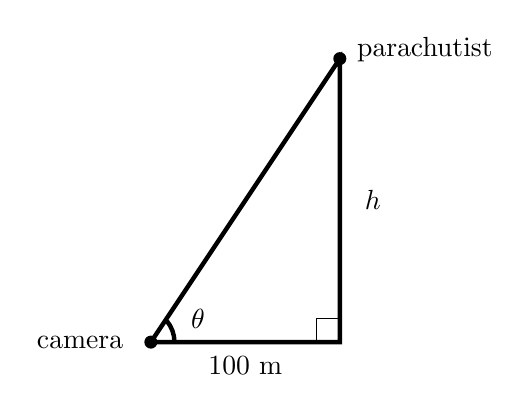
\begin{tikzpicture}[scale=.6]
\draw[ultra thick] (0,0)--(4,0)--(4,6)--(0,0);
\node at (1,0.5){$\theta$};
\draw[ultra thick] (.5,0) arc (0:40:0.7);
\draw (3.5,0)--(3.5,0.5)--(4,0.5);
\node at (2,-.5){ 100 m };
\node at (4.7,3){$h$};
\node at (-1.5,0){camera};
\node[fill,circle,scale=.5] at (4,6){};
\node at (5.8,6.2){parachutist};
\node[fill,circle,scale=.5] at (0,0){};
\end{tikzpicture}

(a) Find an equation relating $h$ and $\theta$ and \textbf{solve it for $\theta.$}
\end{multicols}


	(b) Find $\displaystyle \frac{ d\theta}{dh}.$ (Your answer should use part (a) and should be in terms of $h$.)
	\vfill
	(c) What are the \textbf{units} of $\frac{d\theta}{dh}$?
\vspace{.3in}
\end{enumerate}
\end{document}
\newpage
\item (Extra problem ) Below is the graph of the curve $x^4+y^4+2x^2y=21.$

\includegraphics[scale=.1]{q6pic}
	
	Write an equation of the line tangent to the curve $x^4+y^4+2x^2y=21$ at the point $(2,1)$ and sketch the line in the figure.
	

\end{enumerate}
\end{document}



